\documentclass[11pt]{article} 
\usepackage{geometry}
\usepackage{amsmath}
\usepackage[utf8]{inputenc}
\inputencoding{utf8}
\geometry{a4paper}
\usepackage{graphicx}
\usepackage[table,xcdraw]{xcolor}
\usepackage{pdfpages}
\usepackage{tabu}
\usepackage{longtable}

\graphicspath{{images/}}

\begin{document}

%----------------------------------------------------------------------------------------
%	TITLE PAGE
%----------------------------------------------------------------------------------------

\begin{titlepage}

\newcommand{\HRule}{\rule{\linewidth}{0.5mm}}
\center
\textsc{\LARGE King's College London}\\[1.5cm]
\textsc{\Large Traffic Simulator}\\[0.5cm]
\textsc{\large Group Project}\\[0.5cm]
\HRule \\[0.4cm]
{ \huge \bfseries Team Diversity}\\[0.4cm]
\HRule \\[1.5cm]

\begin{minipage}{0.4\textwidth} \large
\begin{center}
\emph{Members:}\\
Balázs Kiss \\
Eddy Mukasa \\
Yukolthep Visessmit \\
Pongsakorn Riyamongkol \\
Snorri Hannesson
\end{center}
\end{minipage}
\\[2cm]


\includegraphics{KingsLogo}\\[1cm] 

{\large \today}\\[3cm]

\vfill

\end{titlepage}

%----------------------------------------------------------------------------------------
%	Table of contents
%----------------------------------------------------------------------------------------

\tableofcontents

\newpage
%----------------------------------------------------------------------------------------
%	Introduction: Describe the context for the work and the problem you are addressing. Briefly summarise what you achieved in the project.
%----------------------------------------------------------------------------------------

\section{Introduction}
\subsection{Background}
Over the past few decades, the world’s population has been continuously increasing which is becoming a big issues in many countries. This has resulted in overwhelming traffic in the most cities around the world. City planners are therefore looking for ways to solve problems caused by traffic congestion. There are many theories and methods to handle this issues. For example, in Bangkok, priority lanes are used at peak hour to relive traffic congestion.  Above all, any theories and methods which are applied for solving this problem will need to be used together with a good traffic management policy.\\

In this report, we will explain how our traffic simulator works and how the simulator implements two different traffic management policies. These policies can be compared and therefore give implication which policy would be more likely to solve problems in the real world. This traffic simulator are supposed to be an abstract models of the real world, so if a policy works well on the simulator it probably will work well in the real world. This is the reason why traffic simulators are made. 
	
\subsection{Descriptions}
The traffic simulator is an abstract model of actual real world traffic. Roads can have multiple lanes which can go in either direction. The traffic is left lane oriented, as in the UK. The simulator has cars and buses, which differ in size and speed. Drivers can be either cautious, reckless or normal. There are two different traffic management policies fixed time policy and congestion control policy. These policies are compared by average time each vehicle is in the system. Our opinion is that two types of vehicles and three types of driver behaviour gives enough diversity for comparing the different policies, more types of vehicles wouldn't give more accurate results.\\

The simulator will be programmed in Java programming language. The simulator will have a graphical user interface (GUI). The GUI is created with the help of JavaFX software platform. The rational for using a GUI: 1. Better visualisation and understanding of code during development, i.e. actually seeing what is happening when programming. 2. When the final product is ready users can see the road system and the cars and therefore get a better understanding of how the road system is and how the policies work. Opposed to just get the result log and results of which policy is superior and have no visual understanding of what happened. 

\subsection{Objectives}
Our initial objectives for this project where as follows.
\begin{itemize}
\item[•] To develop a traffic simulator program which has the following structure: two types of vehicles, three types of drivers, functional road system with many roads and lanes, junctions, intersections and traffic lights.
\item[•] To compare two different traffic management policies: Fixed Time Policy and Congestion Control Policy.
\item[•]To examine how the system reacts in an emergency period by injecting an ambulance to the simulation.
\end{itemize}

\subsection{Scope}
\begin{itemize}
\item[•] Each road can have multiple lanes, which can be in the same or opposite direction.
\item[•] British traffic is left-lane oriented.
\item[•] The system has only two types of vehicle (cars and buses).
\item[•] There are three types of driver behaviour which is cautious, reckless, and normal.
\end{itemize}
	
\subsection{Methodology}
\begin{itemize}
\item[I.] Analysing: requirement
\item[II.] Planing and Organising: schedule and assigned task
\item[III.] Developing:
	\begin{itemize}
	\item[•] Software: used Java
	\item[•] Source code: stored at GitHub
	\end{itemize}
\item[IV.] 	Evaluating:
	\begin{itemize}
	\item[•] Program
	\item[•] Peer Assessment
	\end{itemize}
\item[V.]  	Reporting:
	\begin{itemize}
	\item[•] Document: written in LaTeX
	\item[•] Presentation
	\end{itemize}
\end{itemize}

\subsection{Schedule}
The development phase (10 weeks) was divided into three iteration. In the first iteration (week 1 to week 4), our team focused on requirement and design. After we had committed to a plan, we started to develop the simulator. In the second iteration (week 5 to week 7) we continued to complete tasks and functions that we had defined as mandatory as well as well as starting to work on implementing the traffic management policies and we started to make unit tests. In the last iteration (week 8 to week 10) much work was done on fine tuning the implementation on the traffic lights and the policies to get correct results. Evaluation of the whole project was also done. However, the emergency strategy was left out due to lack of time. The detail of traffic simulator progress is illustrated in figure 1.      
\begin{center}			
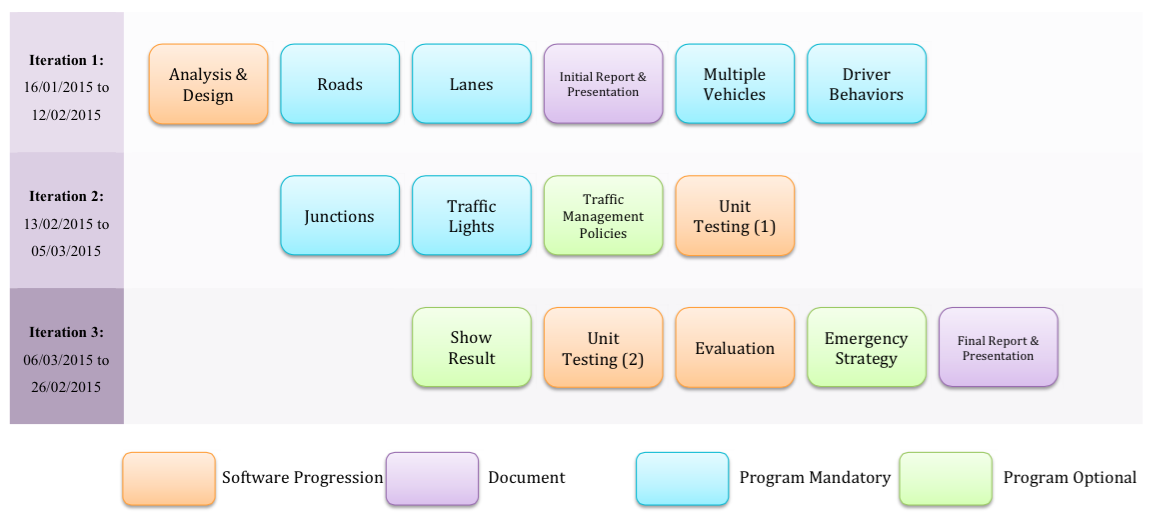
\includegraphics[scale = 0.40]{Figure01}\\
\textit{Figure 1: Schedule}
\end{center}
\subsection{Obstacles}
\begin{description}
\item[Culture and Language]:\\
Our member come four different countries (Hungary, Iceland, Thailand  and Uganda) in three different continents. English isn't the native language for any member. Those cultural and language differences have been an obstacle we have had to face.

Communication is one of the most important aspect for team work. So when we have had a difficult time explaining our thoughts and meaning we have tried to use other means of communication. For instance, pictures and picture drawing have been used a lot to help other members understand some point or a concept.
    
\item[Skill and Background]:\\
The teams members have different skills and background in programming. Some members have worked or are currently working as software developers and some have little experience. However, this project is also about communication, reporting, presentation and more.

We quickly discovered the strengths and weaknesses of each team member. This has always been taken into account when allocating of work. So we have tried to use our strengths to our advantage. We have tried to help each other with tasks, for instance, a member that has much knowledge on some tool helps another member to understand how to use that particular tool. 

\item[Time]:\\
We had only 10 weeks for developing the traffic simulator. That is not a long time if taken into account that team members didn't know each other beforehand.

However, we had a task schedule for each person in deep detail. That helped us to follow up our task and complete the project on time. 
\end{description}

	
\newpage
%----------------------------------------------------------------------------------------
%	Review: Describe related work.
%----------------------------------------------------------------------------------------
\section{Review}
\subsection{Related work}
In today's world a lot of effort is made to make transportation as good as possible. For most countries and cities the road systems is a vital part of it's transportation system. With the ever growing population and increasing purchasing power of the public, good traffic control has never been as urgent. Changes to road systems are hard to make and drivers wouldn't be pleased if many experiments were made on live traffic. That's why traffic simulators play a big role in increasing the quality of the road system. Any change can be simulated and the result of the change can be analysed. There are many challenges that traffic simulation creators face. Trying to predict the behaviour of drivers and the synergistic effects of different factors can have on a driver behaviour is perhaps the most challenging, the goal is to make it as realistic as possible.\\

Many traffic simulators exist as well as many papers and books on that subject. In this module we were given two papers on traffic simulation for inspiration for this project and an insight into this field. Sewall, Wilkie, Merrell and Lin \cite{sewall2010continuum}presented a novel method for the synthesis and animation of realistic traffic flows on large-scale road networks. Their technique is based on a continuum model of traffic flow they extended to correctly handle lane changes and merges, as well as traffic behaviours due to changes in speed limit. They demonstrated how their method can be applied to the animation of many vehicles in a large-scale traffic network at interactive rates and showed that their method can simulate believable traffic flows on publicly available, real-world road data. They furthermore demonstrated the scalability of this technique on many-core systems.\\

Namekawa, F. Ueda, Hioki, Y. Ueda and Satoh \cite{namekawa2005general} spent several years developing a general purpose road-traffic simulation system to analyse road traffic jams. The concept of their system was using the running line model as opposed to fixed road-network information database, which is not effective in their opinion. Their simulator uses the a cell automaton model.
\subsection{Theory}
\begin{itemize}
\item[1. ]\textbf{Driver’s Behaviour:} 
In the report, we categorise the driver’s behaviour into three types (normal, cautious, and reckless). In the program, driver’s behaviour is defined by the speed of the vehicle, as followed.
	\begin{itemize}
	\item[•] Normal: This driver respects the traffic laws, his speed is under the speed limit.  
	\item[•] Cautious: This driver drives slower than normal drivers. He is very careful and avoids danger. 
	\item[•] Reckless: It is obvious that reckless driver drives faster than average speed. It may be overtake the front vehicle or change lanes immediately, does not have much respect for traffic laws. 
  	\end{itemize}	
\item[2. ]\textbf{Passenger Car Unit:}
There are a number of types of vehicle in the traffic which and can vari between locations. Traffic modelling utilises a common unit, know as Passenger Car Unit, to standardise general traffic. SCPtransport \cite{SCPtransport} states that “A Passenger Car Unit (PCU) is a method used in Transport Modelling to allow for the different vehicle types within a traffic flow group to be assessed in a consistent manner.”  TFL (Transport for London) \cite{TFL} is defined PCU value in table 1.\\
\begin{center}			
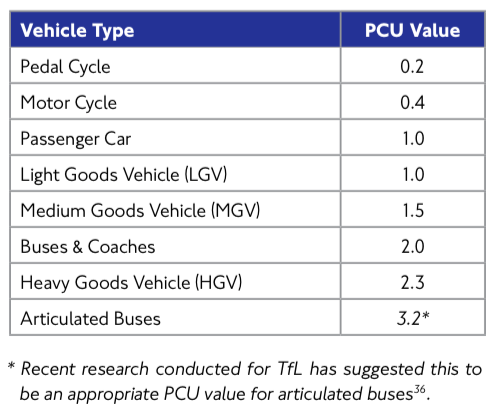
\includegraphics[scale = 0.5]{Figure05}\\
\textit{Table 1: PCU}
\end{center}  	
\item[3. ]\textbf{Road Intersection:}	
According to Andy Chow Lectures 11-12, \cite{Lecture} points out that a road intersection or a junction is a location where multiple roads intersect. This can be divide into five types of intersection, as shown below
	\begin{itemize}
	\item[•] Uncontrolled: no signs or road markings
	\item[•] Roundabouts: traffic circulates around a central island and leaves at a chosen exit
	\item[•] Priority: signs and road markings indicate way
	\item[•] Signal Control: priority as indicated by signal
	\item[•] Grade Separation: conflicting traffic stream, having different level
  	\end{itemize}	
\item[4. ]\textbf{Traffic Signal Lights:}
Traffic Signal or Traffic Lights is a set of coloured lights to control the flow of traffic on the junction. It may use in different meaning or types in another country. In the United Kingdom, the meaning and types is followed
  	\begin{itemize}
	\item[•] RED: stop and wait behind the stop line on the carriageway
	\item[•] RED and AMBER: stop and do not pass through or start until GREEN shows
	\item[•] GREEN: may go on if the way is clear, take special care if you intend to turn left or light and give way to pedestrians who are crossing
	\item[•] AMBER: stop at the stop line, you may go on if the AMBER appears after you have crossed the stop line or are so close to it that to pull up might cause an accident.
	\item[•] GREEN ARROW: same as GREEN but may go on in the arrow sign.
  	\end{itemize}	
\item[5. ]\textbf{Traffic Management Policy:}
In this paper, we will focus on two different traffic management policies— Fixed Time and Congestion Control. Those policies will be compared which one is better by the average time each vehicle spends in the system. Each vehicle will have a timer that starts when it enters the system and gets written to a log when the vehicle exits the system. Therefore, the average time that a vehicle is in the system is calculated and the the policy that generates lower average time is considered better.
	\begin{itemize}
	\item[•] Fixed Time: This is about the peak period and off-peak period during a day which has been applied to a system. The concept of this policy is very simple. In a peak time period, the green light on the desire direction, especially in the business centre area, will be longer than another directions.  And off-peak time period, it will be set the traffic light time equally. which is no one the get more priority.   
	\item[•] Congestion Control: This policy is the policy that automatically changes the duration of the traffic light due to a congestion of the traffic in a simultaneous time. In this programme, the congestion is set by the PCU (Passenger Car Unit) in the road which those vehicle waited. The program will calculate the PCU in every road at this intersection. Suppose that the program has four path—A, B, C, D. If path A has the highest PCU , path A will get a first priority. After the cycle time, the program will calculate the PCU in this junction again.
	\end{itemize}	
\end{itemize}	


\newpage	
%----------------------------------------------------------------------------------------
%	Requirement and Design: Describe the requirements you set for your project at the beginning and the design you have taken for your project. Focus on why you decided to tackle the problem in the way you did, and what effects that had on the design. You may also wish to mention the impact of team-working on your requirements and design.
%----------------------------------------------------------------------------------------	
\section{Requirement and Design}
\subsection{Requirements}
\begin{itemize}
\item[•] The simulation should simulate individual vehicle operating in different parts of a road network
\item[•] The Simulation should have an entry point and exit for vehicles
\item[•] Vehicle should have an entry point and exit points
\item[•] The Simulation should have different individual behaviours for different vehicles
\item[•] The simulation should keep track of vehicles journey
\item[•] The simulation should consider support for emergency services
\item[•] The simulation should compare different time/traffic management policies
\item[•] The simulation should time the duration of the simulation
\item[•] Updates on simulation clock should update all parts of the simulation
\item[•] Simulation engine should record vehicle positions, new entries and exits and other data and update state when moving to the next tick
\end{itemize}

\subsection{Design}
Figure 3 has a UML diagram of the most significant parts of the system. A larger version of this figure can be found in appendix D. \\

\begin{center}
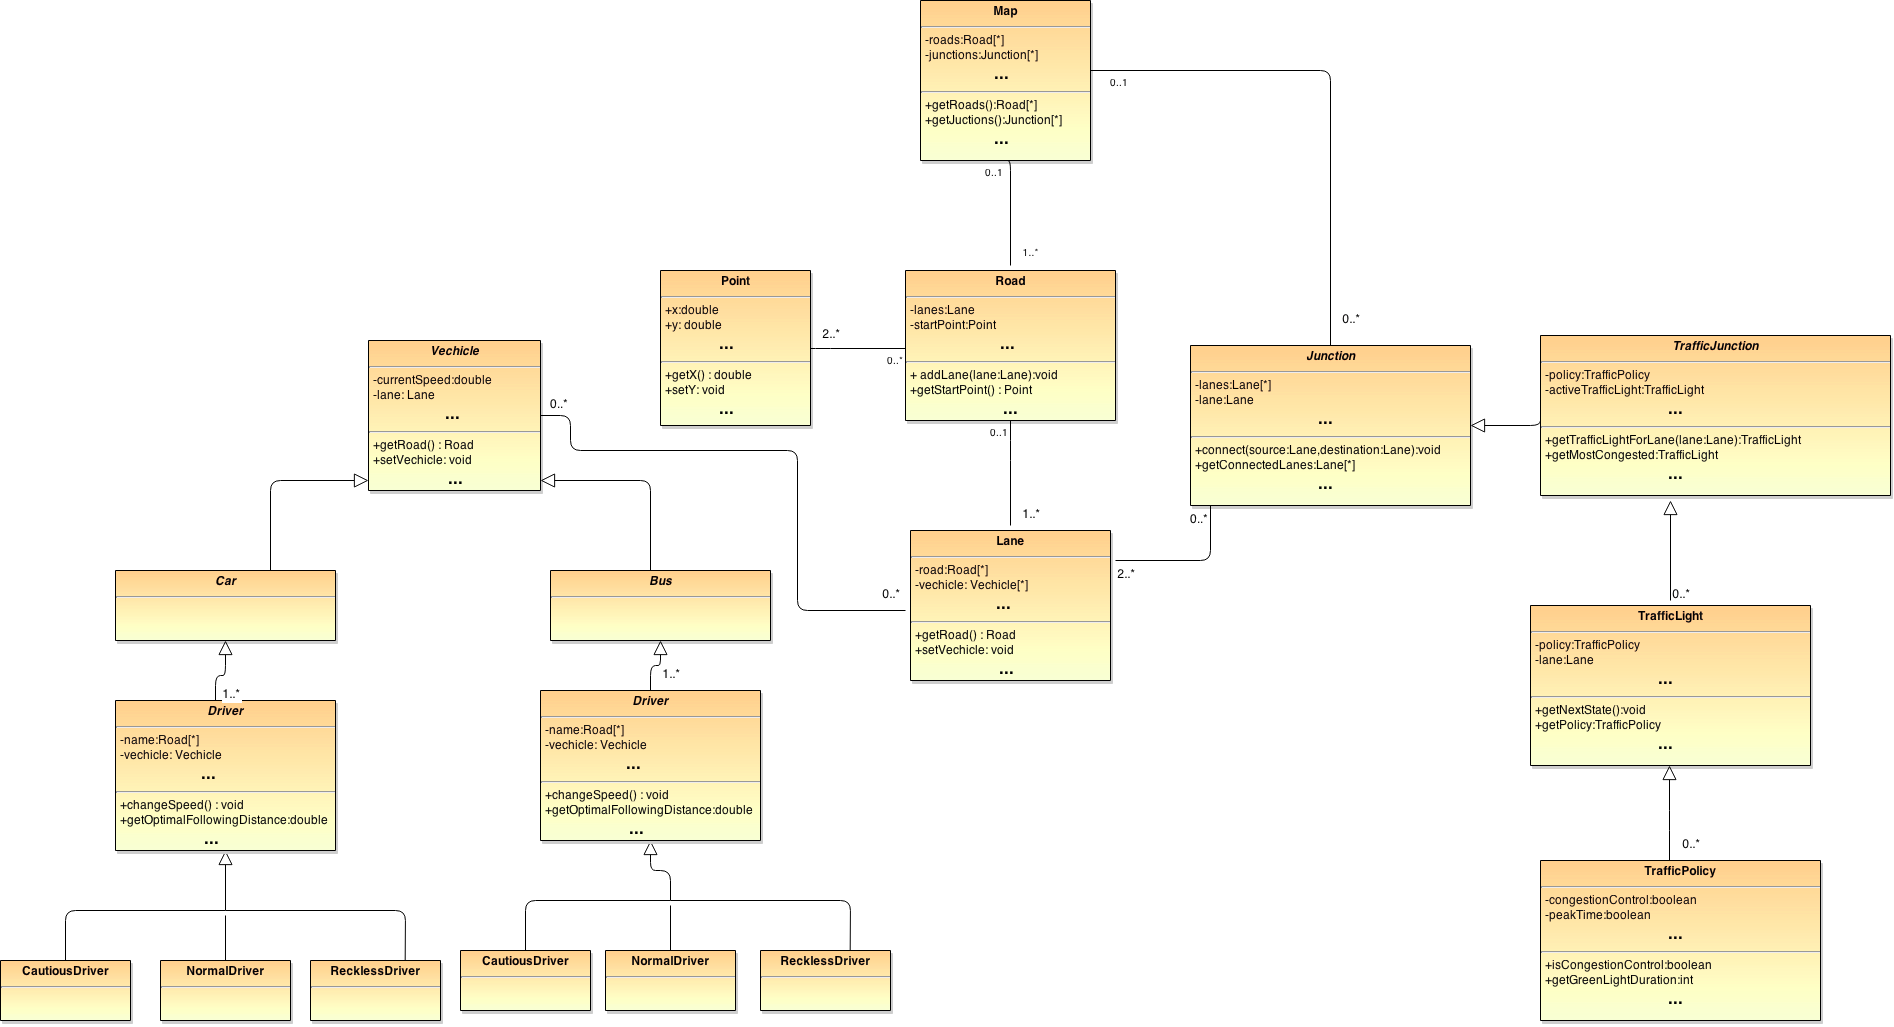
\includegraphics[scale = 0.21]{UML}\\
\textit{Figure 2: UML diagram}
\end{center}

	
	
\newpage
%----------------------------------------------------------------------------------------
%	Implementation: Describe the most significant implementation details, focussing on those where unusual or detailed solutions were required. Quote code fragments wherenecessary, but remember that the full source code will be included as an appendix. Explain how you tested your software (e.g. unit testing) and the extent to which you tested it. If relevant to your project, explain performance issues and how you tackled them.
%----------------------------------------------------------------------------------------
\section{Implementation}
\subsection{Maps}

Modeling the roads is a fundamental part of every traffic simulator software. We have designed ours to be very flexible from the ground up. The four main classes that our program's road model is built upon are:

\begin{description}
  \item[Map] \hfill \\
  A container class for the Road and the Junction classes. The Simulation class requires a Map object.
  \item[Road] \hfill \\
  A road object has a start and an endpoint and can have many lanes. A new lane can be added by calling the addLane(direction) method.
  \item[Lane] \hfill \\
  Vehicles can enter and exit lanes. A lane has a direction that can be identical or opposite to its lane. The position of the lanes are calculated dynamically when it is added to a road object. Drivers can get information about other vehicles from a lane.
  \item[Junction] \hfill \\
  Connects lanes together at the end of the road. The junction class can be subclassed to implement different rules for traffic management. TrafficLightJunction is a subclass that adds traffic lights to every entering lane object.
\end{description}

The following code snippet demonstrates how to set up two roads with two lanes that are connected in a traffic light junction:

\begin{verbatim}
Road road1 = new Road(new Point(0,0), new Point(100,0));
Lane lane1 = road1.addLane(Lane.Direction.IDENTICAL);
Lane lane2 = road1.addLane(Lane.Direction.OPPOSITE);
Road road2 = new Road(new Point(100,100), new Point(100,Lane.LANE_WIDTH*2));
Lane lane3 = road2.addLane(Lane.Direction.IDENTICAL);
Lane lane4 = road2.addLane(Lane.Direction.OPPOSITE);
TrafficLightJunction junction = new TrafficLightJunction(new TrafficPolicy(true, true));
junction.connect(lane1, lane4);
junction.connect(lane2, lane3);
\end{verbatim}

Since the constructor in the road class takes two points, roads can be not only horizontal or vertical but diagonal as well. Furthermore, a road can have any number of lanes. This enabled us to model quite complicated maps for the simulations, but also made the implementation a bit more complicated compared to a grid based solution.

\subsection{Drivers \& Vehicles}
The abstract class Vehicle has all the logic that is needed for the vehicles. The Bus and Car classes inhered from the Vehicle class and these classes pass different values to the Vehicle class. Making cars and buses have different speed, acceleration, deceleration and size. The vehicle class keeps record on what lane it is currently on and also what lane the vehicle will enter at next intersection. The next lane decision is made as soon as the vehicle enters a lane. That makes it easier to keep correct distance between vehicles at intersections.

The abstract class Driver has all the logic that is needed for the vehicles. The CautiousDriver, NormalDriver and RecklessDriver classes inhered from the Driver class and these classes pass different values to the Driver class. Making the different drivers have different acceleration and deceleration.

When initiating a vehicle (car or a bus) a driver, either cautious, normal or reckless needs to be specified.

\subsection{Traffic Policies}

We have designed the system with two traffic policies which are to be set before starting the simulation. These traffic policies are as follows:
\begin{description}
\item[Fixed Time] operates with two configurations peak time and off peak time. During peak time the duration of the green light is twice that of the duration of the green light during off peak time. This is to cater for the increased traffic during peak time
\item[Congestion Control] policy takes into account the number of vehicles on the different lanes at the junction. The justification for this policy is that we have situations in the fixed time policy where we have a green light on an empty lane while some other lane has cars waiting.
\end{description}
These policies are implemented in the traffic junction class and are passed as a parameter to this class’s constructor to ensure that every junction is created with a policy. Below is a code fragment on how to check for congestion:
\begin{verbatim}

private TrafficLight getMostCongested(){
  HashMap<Double, TrafficLight> hm = new HashMap<>();
  for(TrafficLight tf : trafficLights){
    List<Vehicle> vehiclesOnLane = tf.getLane().getVehicles();
    double totalLengthOfVehicle = 0;
            for(Vehicle v : vehiclesOnLane){
             totalLengthOfVehicle = totalLengthOfVehicle + v.getSize().height;
        }
            hm.put(totalLengthOfVehicle,tf);
        }
        Iterator<Double> keySetIterator = hm.keySet().iterator();
        double largest = 0;
        while(keySetIterator.hasNext()){
            Double key = keySetIterator.next();
            if(largest<key){
                largest = key;
            }
        } 
        return hm.get(largest);
  }
  
\end{verbatim}
\subsection{Running the Simulation}

The simulation class plays a central role in the program. It stores a map object and an array of vehicles, and handles the steps of the simulation.\\

On our GUI three different maps (Small Town, New York, London) are available which belong to separate subclasses. In these subclasses the init method is overriden and it creates different maps. Other settings, such as peak time and the selected congestion control policy can be passed to the simulation object.\\

The simulation class contains a timer that is responsible for calling the step() method on its elements. This method is prescribed by the ISteppable interface that is implemented by all the classes that has time dependent behaviour.\\

A number of statistical calculations are also made in this class. For example the shortest, longest and average time spent in the system of the vehicles can be retrieved from here.

\subsection{Testing}
Because the navigation of the user interface is very simple and the system doesn't depend other systems our opinion was that unit testing was the most useful method of testing we could use. For unit testing we used the JUnit library. JUnit is a very easy to use library and has been important in the development of test-driven development (TTD). We set out to use TTD for the most of the project but that was too time consuming so only parts of the project were developed with TTD. The parts that were developed with TDD were the creation of roads and lanes.

\subsection{Graphical User Interface}
In our application, JavaFX is selected as a graphic platform to be used. This platform allows developers to create an application on various platform such as desktop, mobile, or web. Furthermore, this platform introduce the use of cascading style sheets (CSS) to decorate the interface. This way, coders won’t have to worry about decorating the interface themselves in their codes and let CSS designer to handle this instead. Although in our application the use of this benefit haven’t been implemented along with the java code but we think that this is a very helpful technique worth mentioned from JavaFX.\\

Our application consists of 2 stages, which are both a top-level container of JavaFX, one is the main stage that will show a simulation and another one is the one used to show a simulation’s result. The first stage is separated into 2 parts by using Border pane. This pane works like BorderLayout in Javaswing but in JavaFX this layout is implemented into a pane rather than being one of the layout to be set into an empty pane. The followings are put into left and center region of this border pane respectively:
\subsubsection{Main Stage}
The first stage is separated into 2 parts by using Border pane. This pane works like BorderLayout in Javaswing but in JavaFX this layout is implemented into a pane rather than being one of the layout to be set into an empty pane. The followings are put into left and center region of this border pane respectively.
\subsubsection{Canvas}
Canvas is a node that is a blank image. This node can be painted on using GraphicsContext class object. Our canvas has a width of 800 pixels and height of 600 pixels so we don’t have to worry about how our application will run in different screen resolution since this dimension is probably comply with all present screen resolutions.\\

To draw a simulation, we can call a GraphicsContext object from canvas itself using \texttt{getGraphicsContext2D()} and by doing so, we can manipulate the canvas with various methods from GraphicsContext like \texttt{fillPolygon(double[] X, double[] Y)} which will draw a polygon with specified fill colour from a set of coordinate X and Y.\\

To draw roads, we can call an above method and get a set of parameters from a simulation class which contains a list of roads. Each road can provide its own coordinate at each corner so we use this as elements to be added into a set of X and Y coordinate. Because this is a “fill” type method which will also paint an enclosure of a polygon we can provide only 3 points to the method which these are \texttt{leftStartPoint},\texttt{leftEndPoint}, and \texttt{rightEndPoint}. The method automatically close the gap between a start point and last point with a straight line and fill a polygon afterwards.\\

For vehicles, we have already provided a picture for each type of vehicle in a JPEG format and draw these pictures based on what type of vehicle we are dealing with from a list of vehicle provided from simulation class. There is a useful method in Vehicle class called \texttt{getDisplacementVector()}, using this method along with the one in Point class from utils package called \texttt{angleVectorDegree()} we obtain an angle in which a vehicle is running compare to a horizontal line measuring In counter-clockwise manner. After we obtained a value of angle, a method called \texttt{drawRotatedImage()} will do a job to draw a vehicle picture onto a canvas. This method, again, call another method \texttt{rotate()} which receive 4 parameters consist of GraphicsContext object, angle value, x-position, and y-position where these x and y form a coordinate in which will be an anchor point of the rotation. After that, we create a rotate class object by using above parameters. This rotate class object will perform a calculation in order to make a GraphicsContext rotate before we actually draw something using it. After we have rotated the GraphicsContext, we can normally draw a picture onto a canvas. Note that all of these happened after the start button is pressed, which the button will send a signal to start a simulation.
\subsubsection{Settings panel}
In this panel, we take an advantage from JavaFX features called HBox and VBox, which will place objects horizontally and vertically next to previous one by specified insets. The idea is to put many Hboxes into one VBox but since radio buttons still require us to put them in vertically, so we have put one VBox into Hbox to be able to put radio buttons in their correct position. Figure 4 given below will give an overall image of how we put each component together within this pane (HBox indicated by red border, VBox indicated by black border and object are indicated by blue green border).
\\
\begin{center}
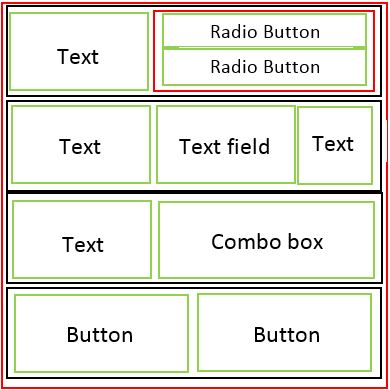
\includegraphics{GUI_component}\\
\textit{Figure 4: HBox and VBox}
\end{center}
\subsubsection{Result stage}
This stage will only appear after the simulation has ended and user press the result button that locates aside of the start button. A simulation will pass various information onto a new stage which will behave as child of the main stage. This means that some behaviour like minimizing and closing will be done to this stage too, if it's happened with its parent. This stage use GridPane which allow us to create a table-liked contents to show to users. A constructor required enough data from a simulation to create a report to user of a current simulation that just has ended.

\newpage
%----------------------------------------------------------------------------------------
%	Team Work: Describe how you worked together, including the tools and processes you used to facilitate group work.
%----------------------------------------------------------------------------------------
\section{Team Work}
In this chapter we'll describe how we worked together during this project, including the tools and processes we used to facilitate group work. We'll will not reflect on what went wrong and what worked well, that is the focus of chapter 6 - Evaluation.
\subsection{Methodology}
A slightly adjusted Agile methodology was used for this project. What is meant be that is we did not follow Agile to the bone but we took bits and pieces from Agile that we knew from previous studies and work experience. The bits and pieces we chose to use from Agile are things that we believed would work for us in this project, i.e. iterations, user stories, roles and we used test driven development to some extend.
\subsubsection{Roles}
\textbf{Balázs Kiss:} Lead programmer\\
\textbf{Eddy Mukasa:} Architect \\
\textbf{Yukolthep Visessmit:} Graphical designer \\
\textbf{Pongsakorn N. Riyamongkol:} Project Manager \\
\textbf{Snorri Hannesson:} Tester and Coordinator \\ \newline
Each member of the group had a responsibility to oversee one aspect of the project but was not expected to do all the work defined in his role. I.e. each member should/could do some programming but the lead programmer should oversee the code and make sure nothing is missing and everything is done properly. The same goes for the other roles.

\subsection{Physical meetings}
Every Thursday at 10 o'clock we had a physical meetings where all team members were expected to attend. We kept log of our meetings so those who were unable to attend the meeting could get up to date by reading the log and for those who did attend the meeting to refresh their memory of what was discussed in the meeting.
In these meetings we discussed the progress we made from last meeting and the problems we were faced with. At the end of each meeting we allocated work to each member witch is supposed to be done during the week until next meeting.
Occasionally extra meetings have been scheduled where a certain aspect of the project been focused on. Not all members are expected to attend these meetings but only the members who are focusing on this certain aspect of the project.
\subsection{GitHub}
Github was used for version control. Our branching strategy was that every time a member wanted to implement a new feature to the system or write something to the report, a new branch was created for that feature. When that branch was created it would be up to date with the master. When work were done on that branch a pull request would be made to the master. The leader of that aspect of the project would then decide to merge or to create a new branch with suggestions of improvements or alterations. Those improvements could then be merged with the original branch which could then be merged with master.
\subsection{Facebook}
Facebook was used as a communication channel. The first thing this team did was to create a facebook group for the team. Most people these days use facebook everyday so this is very convenient communication channel. In this group we would have various discussions about the our progresses or problems. The facebook chat was also used for individual members to discuss matters that were not directly associated to the group as a whole but only the members in the chat.
\subsection{Trello}
Trello is a versatile tool which was used for project management. The rationale for using Trello is that it's very flexible so you can modify the interface to your will. In this project not all tasks were code related which is not a problem when using Trello. 


\newpage
%----------------------------------------------------------------------------------------
%	Evaluation: Critically evaluate your project: what worked well, and what didn’t? how did you do relative to your plan? what changes were the result of improved thinking and what changes were forced upon you? how did your team work together? etc. Note that you need to show that you understand the weaknesses in your work as well as its strengths. You may wish to identify relevant future work that could be done on your project.
%----------------------------------------------------------------------------------------
\section{Evaluation}
In this chapter, we SWOT analysis to evaluate our team and our work. This is very helpful methodology for analysing and evaluating. Moreover, we will then focus on the currents status of the system and future possibilities for the system. Therefore, this evaluation chapter is separated into four parts - our team, our program, current status, and future possibilities.
\subsection{Our Team}
\begin{center}			
	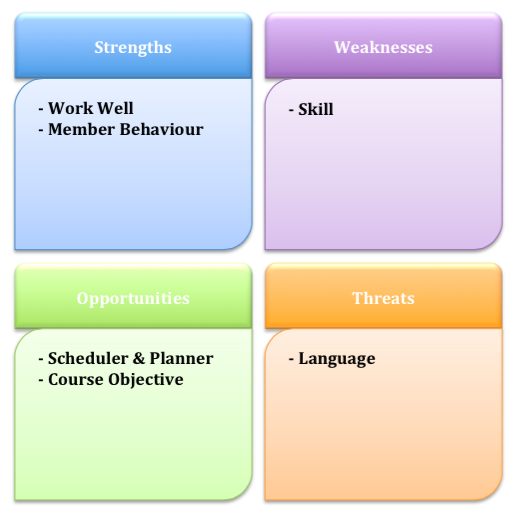
\includegraphics[scale = 0.4]{Figure02}\\
\textit{Figure 3: Team - SWOT}
\end{center}
\begin{description}
\item[Strengths]:
	\begin{itemize}
	\item[•] \underline{Team spirit and mutual respect}: The team have had a good team spirit from day one. That have resulted in good collaboration between team members. This is very positive and is the reason we were able achieve the project goals. In other words, this is our strength and is making us successful in our task. 
	\item[•] \underline{Good work ethics}: This means that each member has been efficient in his work and has shown initiative. Moreover, positive attitude and enthusiasm has been prevailing in this project. Thus, this is the reason why good work ethics has been an advantage point for our team.
  	\end{itemize}				
		
\item[Weaknesses]:
	\begin{itemize}
	\item[•] \underline{Skill}: Because the members of the team have different skills the scenario can happen that a lot of work falls on few hands. Although other team members are eager and willing to help with some task they can't because they don't have the skill set.
	\item[•] \underline{Punctuation and truancy}: During the course of this project we have only had one scheduled meeting per week. It is important that most if not all members attend this meeting, to get up to speed, and be punctual, to get the most of the meeting. Both poor attendance at times and members being late has been a slight problem. 
  	\end{itemize}					

\item[Opportunities]:
	\begin{itemize}
	\item[•] \underline{Scheduler and Planner}: Having only 10 weeks to finish the project forced us to do as good schedule as possible, so we would be able to achieve our goals. That was an opportunity for our team to improve our scheduling and planning skills. 
	\item[•] \underline{Course Objective}: Our members are very appreciative for the opportunity to work as a team. This is very useful for us when working with other people in the future. So, this is an advantage that we can take with us.
  	\end{itemize}				

\item[Threats]:
	\begin{itemize}
	\item[•] \underline{Language}: communication is very important for an effective team, but English isn't the native language of any of our team members. This can result in an misunderstanding. We have been however able to communicate together by using other methods especially pictures, and examples. This means that we have overcome this threat and the team communication has improved during the course of this project.
  	\end{itemize}					
\end{description} 
\newpage
		
\subsection{Our Program}
\begin{center}			
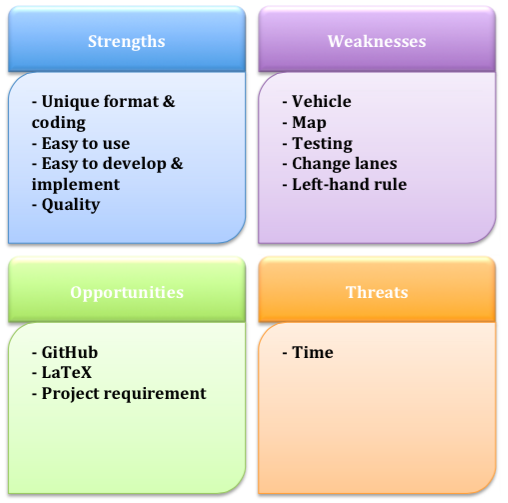
\includegraphics[scale = 0.4]{Figure03}\\
\textit{Figure 4: program - SWOT}
\end{center}

\begin{description}
\item[Strengths]:
	\begin{itemize}
	\item[•] \underline{Unique format and coding}: This Traffic Simulator Program has developed in Java programming language and for GUI is used JavaFX platform. This means that all code in our program is unique and same format. This leads to be easy to run and comply a program; moreover, it is very useful for coding a program when we combine and migrate function in this program together. So our program is written in a same format, structure and language.
	\item[•] \underline{Easy to use}: Our user interface is easy to use and understandable and user friendly.
	\item[•] \underline{Easy to develop and implement}: As the unique format and coding mentioned before, it is the fundamental principle for developing and implementing the program. Our program is very easy to develop and implement due to the unique format and coding. If the next developer would like to develop/change/implement, this system require only Java programming skills. In addition, since our program is written in Java, any platform which support Java is able to implement and run the program as well.
	\item[•] \underline{Quality}: The quality of the code is good. We have tried to follow the simple principles of 'don't repeat yourself' (DRY) and 'keep it simple stupid' (KISS) 
  	\end{itemize}				

\item[Weaknesses]:
	\begin{itemize}
	\item[•] \underline{Vehicle}: The simulator has only two types of vehicles, which is obviously not realistic for the real world wherein many other types of vehicles exist. However, we believe that this isn't a big factor in testing which of our policies is superior. Moreover, how the system is designed it would be very easy to add new types of vehicles if one wanted to do that with future development.
	\item[•] \underline{Map}: We do not use maps that are an exact replica of some place in the real world. This makes the simulator less useful.
	\item[•] \underline{Testing}: We set out to use test-driven development (TDD) for most of the project. Although some aspects of the project were developed with that method most of the program wasn't. This is because of TDD was too time consuming. Moreover, the overall testing of the software isn't at the place we aimed at.
	\item[•] \underline{Change lanes}: Vehicles cannot change lanes.
	\item[•] \underline{No left-hand rule}: We haven't implemented any prioritisation when vehicles meet. That means that only one lane can have a green light at each time on an intersection or else result in many car crashes. 
  	\end{itemize}					

\item[Opportunities]: 
	\begin{itemize}
	\item[•] \underline{Github}: The requirements for this module were to use GitHub for version control. And we are really grateful for that because now we see that Git and Github are very useful and powerful tools.
	\item[•] \underline{LaTex}: The requirements for this module were to use LaTeX for word processing. And we are really grateful for that because now we see that LaTeX much better than other word processing programs.
	\item[•] \underline{Project requirement}: The requirements for this module were develop a simulation engine for testing traffic management policies. These requirements are about vehicles, drivers behaviours, traffic light management, etc. If we had not got these requirements, as mentioned before, our simulator program would not be good. Hence, this was an opportunity for us to show our ability in the programming, teamwork and related useful skills. 
	\end{itemize}				

\item[Threats]:
	\begin{itemize}
	\item[•] \underline{Time}: The limitation of time is an obvious threat that we were faced with in our program. This is because we had only 10 weeks for developing the simulator. It may sound like 10 weeks are enough time to develop the system at first glance, but there are many functions that needs to be considered. This time pressure helped us in the way that we needed to create a precise plan to complete our tasks. Above all, if we have got time more than 10 weeks, we could have created a more sophisticated and better simulator. So, we cannot control this threat and it is difficult to get rid off it.
  	\end{itemize}					
\end{description}
	
\subsection{Current Status}
According to our plan and objectives, we have done all mandatory tasks as well as traffic management policy and show result, that were defined as optional tasks. We didn't have time to make and implement the emergency strategy. The emergency strategy was defined as optional for our traffic simulator program. We tried to follow our plan as much as possible, but some aspects of the program took more time than we expected. This was because of unexpected complications that we hadn't thought of. However, we believe this simulator can give a good implication of which policy is superior.

\subsection{Future Possibilities}
The simulator could be improved with further development in theses aspects: 
\begin{itemize}
\item[•] Emergency Strategy
\item[•] Implement a lane changing method.
\item[•] Implement a prioritisation for vehicles at intersections (left-had rule)
\item[•] Types of vehicle: assign more vehicle (i.e. trucks, motorcycle, bicycle, and van etc.)
\item[•] Real map and traffic route.
\item[•] Adding more or more thought through traffic management polices. 
\end{itemize}


\newpage
%----------------------------------------------------------------------------------------
%	Results: Write about the results of the simulation
%----------------------------------------------------------------------------------------


\section{Result}
After a simulation has ended, we obtain a set of data regarding to that simulation in the result window. Some of these data, especially average time, can be used to analyze the effect of each traffic policy or to compare them between two policies. In traffic management study, we will use the following in order to analyze a simulation or even to the real world.
\subsection{Shortest time}
This data tells users the shortest time for a vehicle to leave the system. A really small value of this type of result does not tell much about the effect of each policy as there might be some vehicles that enter a system with good timing so that they arrive at the junction when a traffic signal for that road turns green. The more that this value getting close to the average time the more it tells us that a policy is working well. The reason behind this logical conclusion is that most of the vehicles that went into the system left the system nearly as fast as the fastest vehicle so when we calculate for the average, the value will be as near as the shortest time if most of the input is very close to the shortest time. Table 2 shows an example of this situation.
\\
\begin{center}
	\begin{tabular}{c c}
		\hline
		Vehicle\# & Time(seconds)\\ \hline
		1 & 18 \\
		2 & 17 \\
		3 & 23 \\
		4 & 21 \\
		5 & 30 \\
		6 & 19 \\
		7 & 17 \\
		8 & 20 \\
		9 & 22 \\
		10 & 18 \\ \hline
	\end{tabular}
	\\[0.1 cm]
	\textit{Table 2: Shortest time}
\end{center}
We can see that the average	time is $ \dfrac{\sum{Time}}{10} $ = 20.5 seconds, which is only 3 seconds more than the shortest time.
\subsection{Longest time}
	In contrast to the shortest time, this data tells users the opposite which is the longest time a vehicle take to leave the system. A really large value in this case can be divided into 2 different situation. First is that, it warns users that a selected traffic management policy may has something wrong since there is at least a single vehicle that has to stay in the system for a long time, compared to the average or not. Second, on the other hand, might happen just because there is a vehicle that appear to stuck twice at the junction where others have already left. Another thing that this value tells us, similarly to the shortest time, is that as this value getting near the average time it can be a sign that our traffic policy that we used to run a simulation is not very effective. Consider again a table like the one above but this time most vehicles will have an average time nearly as long as the longest time.
\\
\begin{center}
	\begin{tabular}{c c}
		\hline
		Vehicle\# & Time(seconds)\\ \hline
		1 & 32 \\
		2 & 30 \\
		3 & 27 \\
		4 & 31 \\
		5 & 30 \\
		6 & 28 \\
		7 & 31 \\
		8 & 29 \\
		9 & 29 \\
		10 & 28 \\ \hline
	\end{tabular}
	\\[0.1 cm]
	\textit{Table 3: Longest time}
\end{center}
This time, the average time is $ \dfrac{\sum{Time}}{10} $ = 29.5 seconds. So most of them took nearly as long as the longest time (32 seconds) in this case.
\subsection{Average time}
	 This is one of the most important factor to be used in analyzing how effective each policy can be. It gives users a broad view of the system as a whole, not specific to a single vehicle. One of the advantage we can take from obtaining this valuable data is that we can make a better decision when there are more than one system to be managed (which always be). Assume the situation that there are three systems in our interest and either two of them can lead to the last one, we can compare their average time simulated with various policies and choose the best result. This result can help drivers to make a decision in which system should they take to reach their destination system as fast as possible.
	 
\newpage	
%----------------------------------------------------------------------------------------
%	Peer Assessment: In a simple table, allocate the 100 ‘points’ you are given to each team member. Valid values range from 0 to 100 inclusive. You may assign decimal values, but the entire points must add up to precisely 100.
%----------------------------------------------------------------------------------------
\section{Peer Assessment}

Robert T. \cite{roberts2006self} states that “The term peer assessment refers to the process of having the learners critically reflect upon, and perhaps suggest grades for, the learning of their peers.” In the other words, peer assessment is a process which student are able to assess their friends based on the criteria. This causes student to provide some feedbacks and evaluate their friends, which may help learning together (University of Reading, \cite{peerAssessment}). Therefore, TeamDiversity is going to use the peer assessment method for grading our member. This will be going to focus on the methodology which is used for assessment following by the criteria. It will be then shown the result and summary of each member in TeamDiversity. 

\subsection{How do we evaluate our member?}	
\begin{itemize}
\item[I.] Distribute the assessment form and assessment criteria to our member.
\item[II.] In each member, he/she must score himself/herself as well as other group member. For example, if our team has 4 people, it will grade 1 for yourself and 3 for our friends.
\item[III.] When you have completed a score (your friends and yourself), you need to mark total add up all scores and calculate the average score for yourself.
\item[IV.] We use only the average score to evaluate our friends and present in this report. 
\end{itemize}

\subsection{What is the criteria that we have used?}
University of Sydney \cite{AssessmentCiteria} has published the assessment criteria and form on the website. TeamDiversity has adapted both documents in the appropriate way for supporting our task. This criteria is going to evaluate ten aspects of member behaviour. In each aspect, we have scored in the range from 0—10. Thus, the total marks of each member will vary from 0—100 inclusive. There will be then illustrated the detail in each aspect of peer assessment criteria, as followed \newline

\textbf{A. Quantity of Work:}\\
	\indent\indent 0	- not taking part in it, having no prospect of progress/value \\
	\indent\indent 1—2	- doing a particular, not too much but enough\\
	\indent\indent 3—4	- sometimes above standard, generally needs improvement \\
	\indent\indent 5—6	- satisfactory, doing more than requirement \\
	\indent\indent 7—8	- always working hard and consistent \\
	\indent\indent 9—10	- outstanding, always over productivity standards \\

\textbf{B. Quality of Work:}\\
	\indent\indent 0	- not giving sufficient attention, making frequent mistakes\\
	\indent\indent 1—2	- giving attention, making some mistakes\\
	\indent\indent 3—4	- doing well, basically correct\\
	\indent\indent 5—6	- satisfactory, accurate in some aspect\\
	\indent\indent 7—8	- almost accurate in all involving fields\\
	\indent\indent 9—10	- outstanding, perfect work\\

\textbf{C. Communication Skills:}\\
	\indent\indent 0	- having bad manners, not showing respect for other people, not listen\\
	\indent\indent 1—2	- friendly and easy to talk to once know by others\\
	\indent\indent 3—4	- warm and friendly, sociable\\
	\indent\indent 5—6	- showing good manners, kindly, listens and understands\\
	\indent\indent 7—8	- courteous and respectful, best wish\\ 
	\indent\indent 9—10	- Inspiring to others, excellent at listening and understanding\\

\textbf{D. Initiative:}\\
	\indent\indent 0	- acts without plan/purpose\\
	\indent\indent 1—2	- need encouragement to do task\\
	\indent\indent 3—4	- putting in minimal effort to complete task\\
	\indent\indent 5—6	- desire to achieve task/goal\\
	\indent\indent 7—8	- strongly desire to achieve task/goal\\
	\indent\indent 9—10	- beyond duty, high motivation\\

\textbf{E. Efficiency:}\\
	\indent\indent 0	- always delayed\\
	\indent\indent 1—2	- occasionally finished on time\\  
	\indent\indent 3—4	- usually finished on time, having minor errors\\
	\indent\indent 5—6	- always finished on time\\
	\indent\indent 7—8	- absolutely completed, consistent in troubleshooting and solving major problems\\ 
	\indent\indent 9—10	- invariably completed ahead of schedule, showing creativity, making major contributions\\ 

\textbf{F. Personal Relations:}\\
	\indent\indent 0	- very disruptive influence\\
	\indent\indent 1—2	- some friction\\
	\indent\indent 3—4	- no problem, commonly\\
	\indent\indent 5—6	- satisfactory, tuneful, harmonious\\ 
	\indent\indent 7—8	- positive factor\\
	\indent\indent 9—10	- respect by others\\

\textbf{G. Group Meeting Attendance:}\\
	\indent\indent 0	- never attended to meeting, not interest\\
	\indent\indent 1—2	- sometime attended \\
	\indent\indent 3—4	- usually attended, hard to get touch with\\
	\indent\indent 5—6	- attend, normally late\\
	\indent\indent 7—8	- count on to attend\\
	\indent\indent 9—10	- never ever missed a meeting, on time\\

\textbf{H. Attitude and Enthusiasm:}\\
	\indent\indent 0	- low disposition, having no prospect of value, unconcerned \\
	\indent\indent 1—2	- feeling/showing few excitement, blasé\\
	\indent\indent 3—4	- half hearted \\
	\indent\indent 5—6	- positive outward behaviour/bearing\\
	\indent\indent 7—8	- positive attitude and spirited\\
	\indent\indent 9—10	- excitement and eager, inspiring to others, positive thinking and influence\\

\textbf{I. Effort:}\\
	\indent\indent 0	- expects others to carry the load\\
	\indent\indent 1—2	- leave some effort\\
	\indent\indent 3—4	- displays enough endeavour\\
	\indent\indent 5—6	- firm and stable contributions\\
	\indent\indent 7—8	- energetic\\
	\indent\indent 9—10	- self starter, normally beyond duty\\

\textbf{J. Dependability:}\\ 
	\indent\indent 0	- unreliable\\
	\indent\indent 1—2	- unsteady, but slightly dependability \\
	\indent\indent 3—4	- inconsistent, occasionally be\\
	\indent\indent 5—6	- suitable, need some improvement \\
	\indent\indent 7—8	- very trustworthy, responsibility \\
	\indent\indent 9—10	- always responsible, steady influence

\subsection{Result and summary of peer assessment?}
\begin{center}			
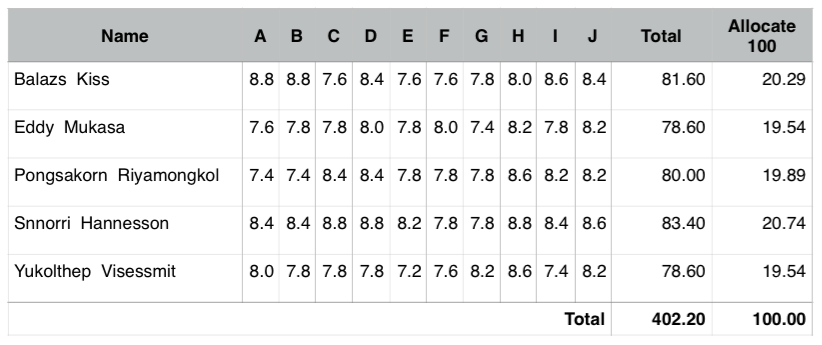
\includegraphics[scale = 0.5]{Figure04}\\
\textit{Table 4: Peer assessment}
\end{center}

\newpage	
%----------------------------------------------------------------------------------------
%	References
%----------------------------------------------------------------------------------------
\bibliographystyle{plain}
\bibliography{References}


\newpage	
%----------------------------------------------------------------------------------------
%	Appendices
%----------------------------------------------------------------------------------------
\addtocontents{toc}{\vspace{2em}}

\appendix
% Appendix A: the Gitlog

\section{Gitlog}
\label{AppendixA}

\begin{center}
\begin{longtabu} to \textwidth {|
    X[4,l]|
    X[3,c]|
    X[8,l]|}
    \hline
    \textbf{Author} & \textbf{Date} & \textbf{Message} \\ \hline
Balázs Kiss & 2015-01-25 & Initial architecture \\ \hline
Balázs Kiss & 2015-01-26 & Ignore build directory \\ \hline
snh11 & 2015-01-26 & Meeting log created, first three meetings documented \\ \hline
Snorrihann & 2015-01-26 & A template for the initial report \\ \hline
Snorrihann & 2015-01-28 & More work done on the intital report \\ \hline
Snorrihann & 2015-01-29 & Modification of roles \\ \hline
Snorrihann & 2015-01-29 & sdfsf dfsd ds \\ \hline
Snorrihann & 2015-01-29 & Change to conflicts \\ \hline
Snorri Hannesson & 2015-01-29 & Merge pull request \#1 from teamDiversity/Snorri\_Conflicts \\ \hline
Balázs Kiss & 2015-02-01 & Speed model for vehicles, basic collison avoidance \\ \hline
Balázs Kiss & 2015-02-01 & Merge pull request \#2 from teamDiversity/develop\_speed \\ \hline
Snorrihann & 2015-02-03 & meeting 29th of january \\ \hline
Snorri Hannesson & 2015-02-03 & Merge pull request \#3 from teamDiversity/meeting\_log \\ \hline
Snorrihann & 2015-02-04 & Implementation of different types of vehicles \\ \hline
Snorrihann & 2015-02-04 & Changes on the initial report made by Neab \\ \hline
Snorri Hannesson & 2015-02-04 & Merge pull request \#4 from teamDiversity/initialReport\_NeabChanges \\ \hline
Snorri Hannesson & 2015-02-04 & Update .gitignore \\ \hline
Snorri Hannesson & 2015-02-04 & Delete initialReport.txt \\ \hline
Snorri Hannesson & 2015-02-04 & Delete initialReport.wc \\ \hline
Balázs Kiss & 2015-02-05 & Corrected my name \\ \hline
Balázs Kiss & 2015-02-05 & Merge pull request \#5 from teamDiversity/report\_typo \\ \hline
Balázs Kiss & 2015-02-05 & Removed junk \\ \hline
Balázs Kiss & 2015-02-05 & Merge pull request \#6 from teamDiversity/report\_typo \\ \hline
Balázs Kiss & 2015-02-05 & Moved vehicle classes to separate package \\ \hline
Balázs Kiss & 2015-02-05 & Use protected topSpeed field for vehicles \\ \hline
Snorrihann & 2015-02-05 & Merge branch `develop\_carsAndBuses\_improvements' of https://github.com/teamDiversity/trafficSim \\ \hline
Snorrihann & 2015-02-05 & Succestions of improvements implemented \\ \hline
yukolthep & 2015-02-05 & first gui implementation \\ \hline
Balázs Kiss & 2015-02-05 & Merge pull request \#9 from teamDiversity/master \\ \hline
Snorrihann & 2015-02-05 & meeting 5th of feb \\ \hline
Snorri Hannesson & 2015-02-05 & Merge pull request \#7 from teamDiversity/develop\_carsAndBuses\_improvements \\ \hline
Snorri Hannesson & 2015-02-05 & Merge pull request \#10 from teamDiversity/develop\_carsAndBuses \\ \hline
Snorrihann & 2015-02-05 & Merge branch `master' of https://github.com/teamDiversity/trafficSim \\ \hline
Snorrihann & 2015-02-05 & acceleration re-changed to maxAcceleration \\ \hline
Snorri Hannesson & 2015-02-05 & Merge pull request \#11 from teamDiversity/development\_maxAcceleration \\ \hline
Snorrihann & 2015-02-05 & Meeting 5th feb logged \\ \hline
Snorri Hannesson & 2015-02-05 & Merge pull request \#13 from teamDiversity/meeting\_5thFeb \\ \hline
Snorrihann & 2015-02-05 & The mandatory/optional table and some proofreading \\ \hline
Balázs Kiss & 2015-02-07 & These files were not the latest \\ \hline
Balázs Kiss & 2015-02-07 & Merge branch `master' into gabb\_branch\_merge \\ \hline
Balázs Kiss & 2015-02-07 & put back maxAcceleration \\ \hline
Balázs Kiss & 2015-02-07 & Merged vehicle subclasses \\ \hline
Balázs Kiss & 2015-02-07 & Changed project type to Java FX \\ \hline
Balázs Kiss & 2015-02-07 & Cleanup \\ \hline
Balázs Kiss & 2015-02-07 & Merge pull request \#14 from teamDiversity/gabb\_branch\_merge \\ \hline
Balázs Kiss & 2015-02-07 & Simulation classes \\ \hline
Balázs Kiss & 2015-02-07 & Removed unnecessary parts from GUISimulation class \\ \hline
Balázs Kiss & 2015-02-07 & Merge pull request \#15 from teamDiversity/simulation\_classes \\ \hline
Balázs Kiss & 2015-02-07 & Small changes \\ \hline
Balázs Kiss & 2015-02-07 & Merge pull request \#16 from teamDiversity/initial\_report\_balazs \\ \hline
Pongsakorn N. Riyamongkol & 2015-02-08 & 1. This is the same as InitialReport.tex 2. If i edit, it is in this pool 3. I will put presentation slide too \\ \hline
Snorrihann & 2015-02-09 & Changes made on the meeting 9 feb \\ \hline
Snorri Hannesson & 2015-02-09 & Merge pull request \#17 from teamDiversity/intialReport\_changesFromMeeting9Feb \\ \hline
Snorrihann & 2015-02-09 & Meeting log 9th of feb \\ \hline
Snorrihann & 2015-02-09 & Changes made to fit requirements on the `Nodes on the inital report' \\ \hline
Snorri Hannesson & 2015-02-09 & Merge pull request \#18 from teamDiversity/meeting\_9thFeb \\ \hline
Snorri Hannesson & 2015-02-09 & Merge pull request \#19 from teamDiversity/intialReport\_changesFromMeeting9Feb \\ \hline
eddymukasa & 2015-02-10 & UML Use case and Class diagram \\ \hline
eddymukasa & 2015-02-10 & Updates to UML Class multiplicities \\ \hline
eddymukasa & 2015-02-10 & Merge pull request \#20 from teamDiversity/UMLDesigns \\ \hline
eddymukasa & 2015-02-10 & Updates to UML Class multiplicities \\ \hline
eddymukasa & 2015-02-10 & merge conflict resolution \\ \hline
eddymukasa & 2015-02-10 & new class diagram \\ \hline
yukolthep & 2015-02-11 & update on car's picture \\ \hline
Balázs Kiss & 2015-02-11 & Merge branch `UMLDesigns' \\ \hline
Balázs Kiss & 2015-02-11 & Merge branch `master' into develop\_gui \\ \hline
Balázs Kiss & 2015-02-11 & Renderer classes, code cleanup \\ \hline
Balázs Kiss & 2015-02-11 & Fixed thread synch bug \\ \hline
Balázs Kiss & 2015-02-11 & Better map for testing \\ \hline
Snorrihann & 2015-02-12 & First tests, just for fun \\ \hline
Snorri Hannesson & 2015-02-12 & Merge pull request \#22 from teamDiversity/test\_basicInitialTestSuite \\ \hline
yukolthep & 2015-02-16 & draw horizontal and vertical roads, still rotated road left \\ \hline
Snorrihann & 2015-02-18 & More tests on vehicle and road system and a test suite class created \\ \hline
Snorri Hannesson & 2015-02-18 & Merge pull request \#23 from teamDiversity/test\_basicFunctions \\ \hline
Snorrihann & 2015-02-18 & jUnit library added to project.properties \\ \hline
Snorrihann & 2015-02-18 & jUnit library added to project.properties \\ \hline
Snorrihann & 2015-02-18 & meeting log updated \\ \hline
Snorri Hannesson & 2015-02-18 & Merge pull request \#25 from teamDiversity/meeting\_11feb \\ \hline
Snorrihann & 2015-02-19 & First creation of final report \\ \hline
Snorri Hannesson & 2015-02-19 & Merge pull request \#26 from teamDiversity/finalReport\_SnorriInitialWork \\ \hline
Snorri Hannesson & 2015-02-19 & Merge pull request \#24 from teamDiversity/test\_jUnitLibrary \\ \hline
Snorrihann & 2015-02-19 & meeting 19feb \\ \hline
Snorri Hannesson & 2015-02-19 & Merge pull request \#27 from teamDiversity/meeting\_19feb \\ \hline
yukolthep & 2015-02-19 & try some manual drawing. still have problem with wrong drawing of rotated road. The angle calculated using the formula seems to be correct but after draw the rotated rectangular with specified angle, it is not correct as the road is drawn with wrong angle. Still can't figure out what is the cause. \\ \hline
eddymukasa & 2015-02-19 & Adding driver Classes to project \\ \hline
eddymukasa & 2015-02-19 & CautiousDriver fix \\ \hline
yukolthep & 2015-02-20 & - fix drawVehicle to correctly draw car using correct angle. - Simulation2 class is used for testing different rotated roads drawing \\ \hline
Snorrihann & 2015-02-20 & Roads and lanes now have four points as a paramiter: leftStart, rightStart, leftEnd, rightEnd. Roads are initialised by the leftStart and leftEnd. \\ \hline
Balázs Kiss & 2015-02-21 & Project properties \\ \hline
Balázs Kiss & 2015-02-21 & step counter \\ \hline
Balázs Kiss & 2015-02-21 & Removed vehicle position from constructor \\ \hline
Balázs Kiss & 2015-02-21 & inherited type method \\ \hline
Balázs Kiss & 2015-02-21 & Removed lane from constructor \\ \hline
Balázs Kiss & 2015-02-21 & Removed unneded methods \\ \hline
Balázs Kiss & 2015-02-21 & Vehicles added at entrypoint \\ \hline
Balázs Kiss & 2015-02-21 & vehicles exit the system \\ \hline
Balázs Kiss & 2015-02-21 & Simualtion stops when all cars exited the system \\ \hline
Balázs Kiss & 2015-02-21 & Passing tests \\ \hline
Balázs Kiss & 2015-02-21 & Merge pull request \#28 from teamDiversity/entry\_and\_exit\_points \\ \hline
Balázs Kiss & 2015-02-21 & Merge development\_widthOfLanes \\ \hline
Balázs Kiss & 2015-02-21 & Merge development\_widthOfLanes \\ \hline
Balázs Kiss & 2015-02-22 & Merge branch `development\_widthOfLanes' \\ \hline
yukolthep & 2015-02-23 & - added new simple car and bus image. - draw vehicles based on their type. - fixed Normal and Cautious bus to extend from Bus class instead of Car class. \\ \hline
yukolthep & 2015-02-23 & - fixed using class instead of string to decide what type of vehicle it is \\ \hline
yukolthep & 2015-02-23 & - changed canvas size back to 800x600 \\ \hline
yukolthep & 2015-02-27 & - clean up some unused test code - bug in drawing a car with wrong position possibly caused by the position of vehicle itself as the position reading from a command line is wrong. need further investigation. \\ \hline
Snorrihann & 2015-02-28 & roads and lanes tested \\ \hline
Snorrihann & 2015-02-28 & bugs fixed in Road and Lane classes \\ \hline
Snorrihann & 2015-02-28 & minor fix on Lane \\ \hline
eddymukasa & 2015-03-01 & Implementing driver logic \\ \hline
Pongsakorn N. Riyamongkol & 2015-03-01 & \ldots{}. \\ \hline
Balázs Kiss & 2015-03-02 & Merge branch `finalReport\_IntNeab' \\ \hline
Balázs Kiss & 2015-03-02 & Merge branch `gui\_draw\_vehicles\_with\_correct\_size' \\ \hline
Balázs Kiss & 2015-03-02 & jfxrt in project description file \\ \hline
Balázs Kiss & 2015-03-02 & Merge branch `test\_RoadsLanes' \\ \hline
Balázs Kiss & 2015-03-02 & Fixed syntax errors \\ \hline
Snorrihann & 2015-03-02 & incorrect pos when road has slope \\ \hline
Snorrihann & 2015-03-02 & centerPoints for start and end \\ \hline
eddymukasa & 2015-03-04 & driverLogic fix \\ \hline
Snorrihann & 2015-03-04 & time for vehicles in system printed in console \\ \hline
yukolthep & 2015-03-04 & - add start button - implement the program to automatically stop after closing the window \\ \hline
Pongsakorn N. Riyamongkol & 2015-03-05 & meeting 26th of feb \\ \hline
Pongsakorn N. Riyamongkol & 2015-03-05 & meeting 26th of feb logged \\ \hline
Snorri Hannesson & 2015-03-05 & Merge pull request \#38 from teamDiversity/meeting\_26thfeb \\ \hline
Pongsakorn N. Riyamongkol & 2015-03-05 & outline of final report \\ \hline
Snorri Hannesson & 2015-03-05 & Merge pull request \#39 from teamDiversity/finalReport\_NeabInitialWork \\ \hline
Snorrihann & 2015-03-05 & meeting 5th of march logged \\ \hline
Snorri Hannesson & 2015-03-05 & Merge pull request \#40 from teamDiversity/meeting\_5thmarch \\ \hline
Snorrihann & 2015-03-05 & cleanup \\ \hline
Snorri Hannesson & 2015-03-05 & Merge pull request \#41 from teamDiversity/snorri\_cleanup \\ \hline
Balázs Kiss & 2015-03-06 & Merge commit `c12333d2b4a4e92263268e834ad0e56c0417e108' \\ \hline
Balázs Kiss & 2015-03-06 & Merge branch `master' into driver\_logic\_merge \\ \hline
Balázs Kiss & 2015-03-06 & updated gitignore file \\ \hline
Balázs Kiss & 2015-03-06 & Fixing incompatibilities \\ \hline
Balázs Kiss & 2015-03-06 & Default constructor for vehicles \\ \hline
Balázs Kiss & 2015-03-06 & format code \\ \hline
Balázs Kiss & 2015-03-06 & Merge commit `8f5224a3bfea688218a80388091d5406e923f386' \\ \hline
Balázs Kiss & 2015-03-06 & formatting \\ \hline
Balázs Kiss & 2015-03-06 & Renamed package \\ \hline
Balázs Kiss & 2015-03-06 & Removed private netbeans files \\ \hline
Balázs Kiss & 2015-03-06 & Default speeds \\ \hline
Balázs Kiss & 2015-03-06 & Removed unused imports \\ \hline
Balázs Kiss & 2015-03-06 & Removed vehicle properties from driver classes \\ \hline
Balázs Kiss & 2015-03-07 & Moved decision methods to driver \\ \hline
Balázs Kiss & 2015-03-07 & driver dependant deceleration \\ \hline
Balázs Kiss & 2015-03-07 & dont round new positions \\ \hline
Balázs Kiss & 2015-03-07 & draw lanes \\ \hline
Balázs Kiss & 2015-03-07 & Added basic classes \\ \hline
Balázs Kiss & 2015-03-07 & steppable, traffic light states \\ \hline
Balázs Kiss & 2015-03-07 & add junctions to simulation \\ \hline
Balázs Kiss & 2015-03-08 & Merge branch `master' into gui\_create\_start\_button\_merge \\ \hline
yukolthep & 2015-03-08 & - change draw road to fillPolygon() which does not need to calculate anything \\ \hline
yukolthep & 2015-03-08 & - edit car and bus images (rotate 90 deg) - made getDisplacementVector() public for using in SimulationRenderer class - implement new way to draw vehicles - add angleVectorDegree which returns in degree instead of radian \\ \hline
yukolthep & 2015-03-08 & - remove testing code \\ \hline
yukolthep & 2015-03-08 & Merge pull request \#43 from teamDiversity/gui\_rework\_on\_drawing \\ \hline
yukolthep & 2015-03-08 & - add a new class which will show a result of a simulation (left blank for now) \\ \hline
Snorri Hannesson & 2015-03-08 & Merge pull request \#44 from teamDiversity/gui\_add\_more\_user\_interface \\ \hline
yukolthep & 2015-03-08 & - add radio buttons group to specify policy to be used - add textbox for user to enter duration of a simulation - add combobox for user to choose from pre-defined maps \\ \hline
yukolthep & 2015-03-08 & Merge pull request \#45 from teamDiversity/gui\_add\_more\_user\_interface \\ \hline
yukolthep & 2015-03-08 & - add show result button \\ \hline
Snorri Hannesson & 2015-03-08 & Merge pull request \#46 from teamDiversity/gui\_add\_result\_window\_button \\ \hline
Snorrihann & 2015-03-08 & results \\ \hline
Snorri Hannesson & 2015-03-08 & Merge pull request \#47 from teamDiversity/development\_results \\ \hline
Snorrihann & 2015-03-11 & Chapter Related work written \\ \hline
Snorri Hannesson & 2015-03-11 & Merge pull request \#49 from teamDiversity/finalReport\_ChapterRelatedWork\_1 \\ \hline
Balázs Kiss & 2015-03-12 & merged tex file \\ \hline
Snorrihann & 2015-03-12 & appendix change \\ \hline
Snorri Hannesson & 2015-03-12 & Merge pull request \#52 from teamDiversity/finalReport\_appendixtemplatechange \\ \hline
\end{longtabu}
\end{center}







\newpage
% Appendix B: the source code

\section{Source Code}
\label{AppendixB}

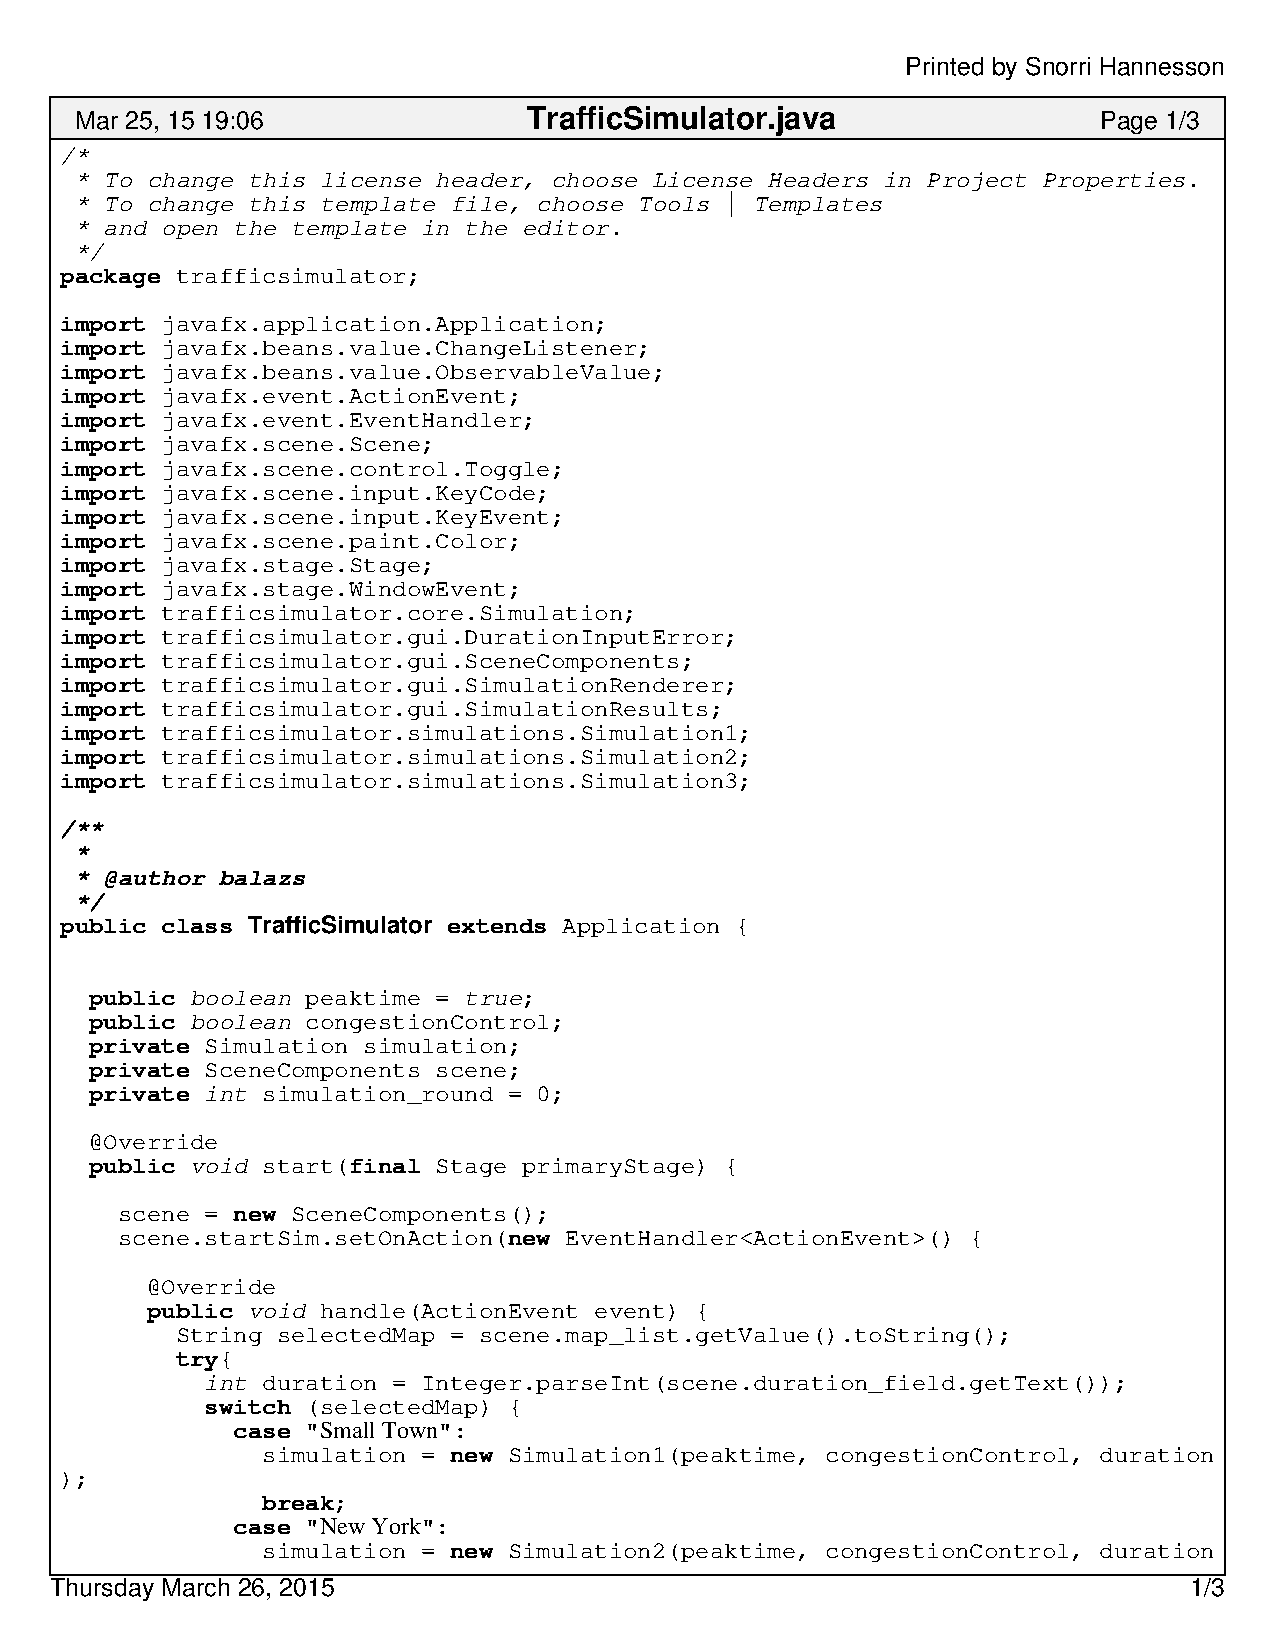
\includepdf[pages=-]{Appendices/code/sim.pdf}
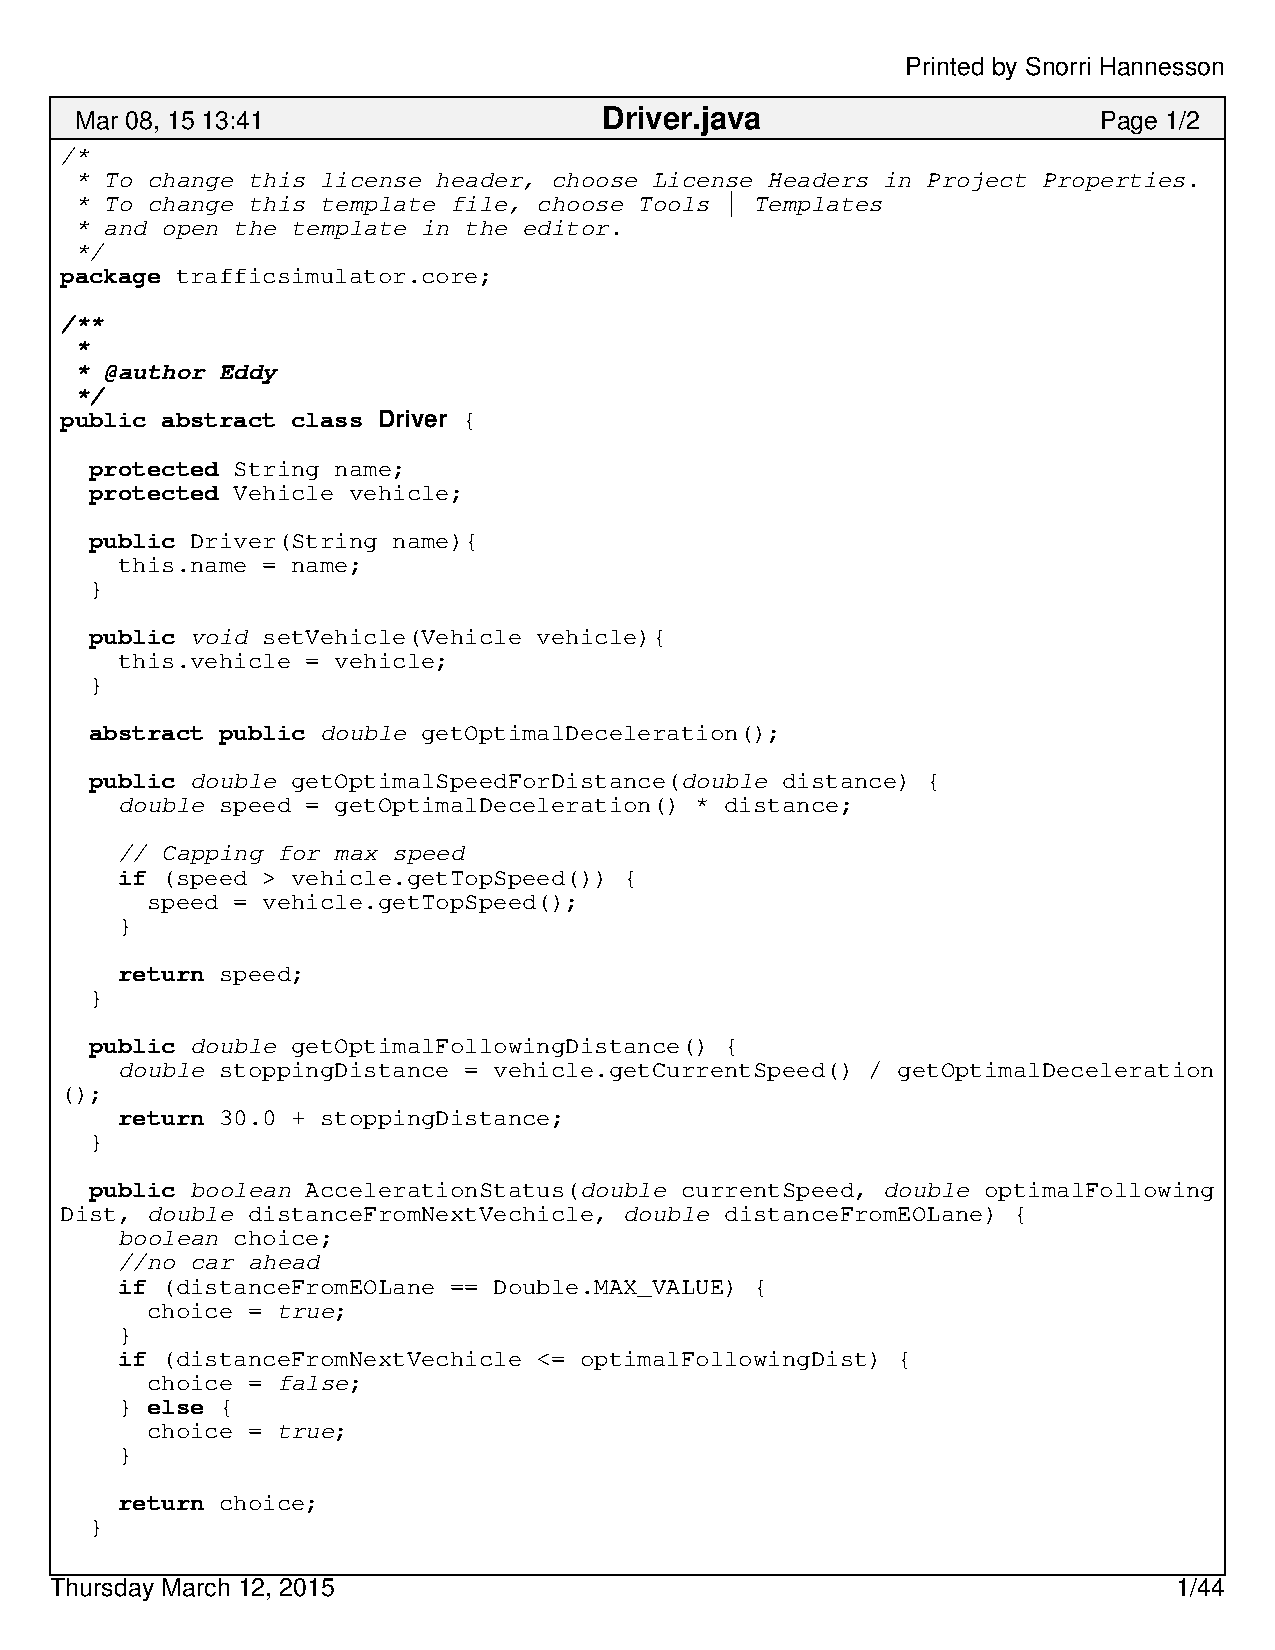
\includepdf[pages=-]{Appendices/code/core.pdf}
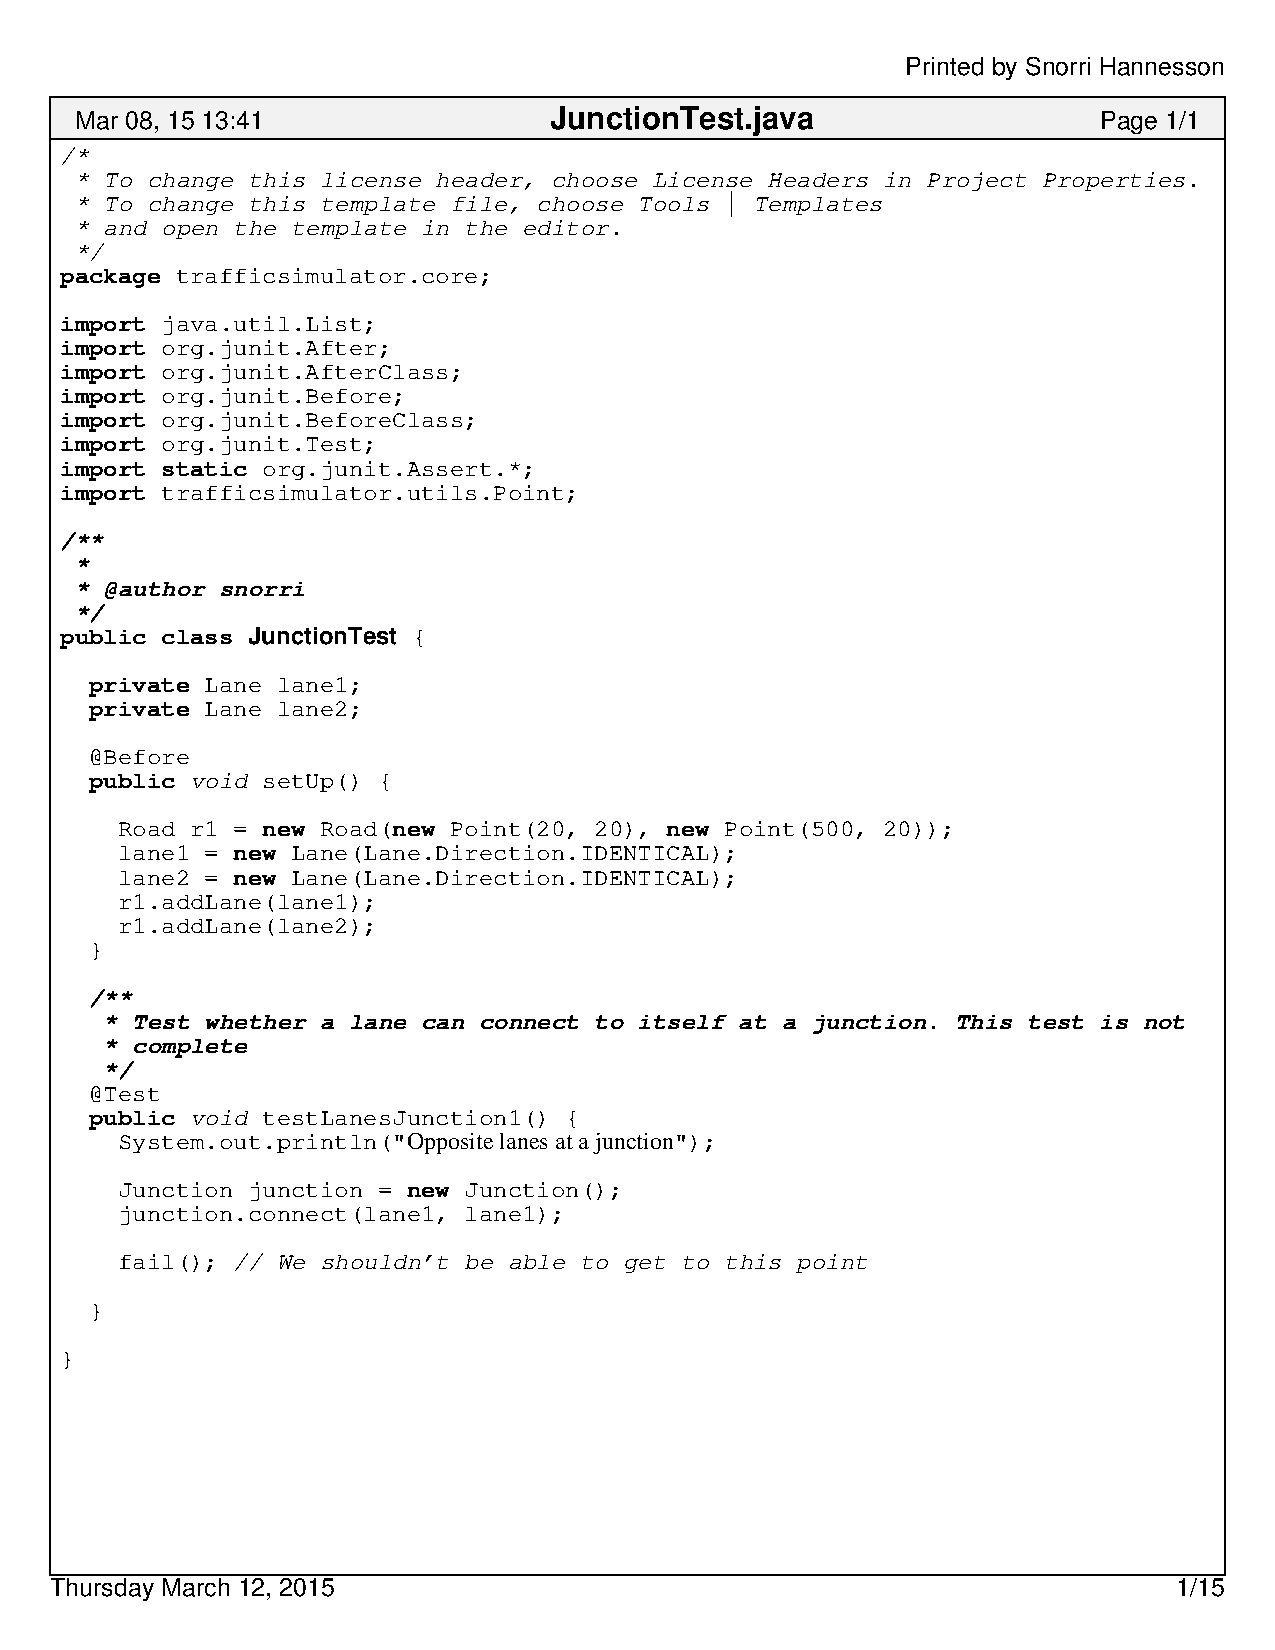
\includepdf[pages=-]{Appendices/code/tests.pdf}
\newpage
% Appendix C: Peer assesment forms

\section{Assessment forms}
\label{AppendixC}

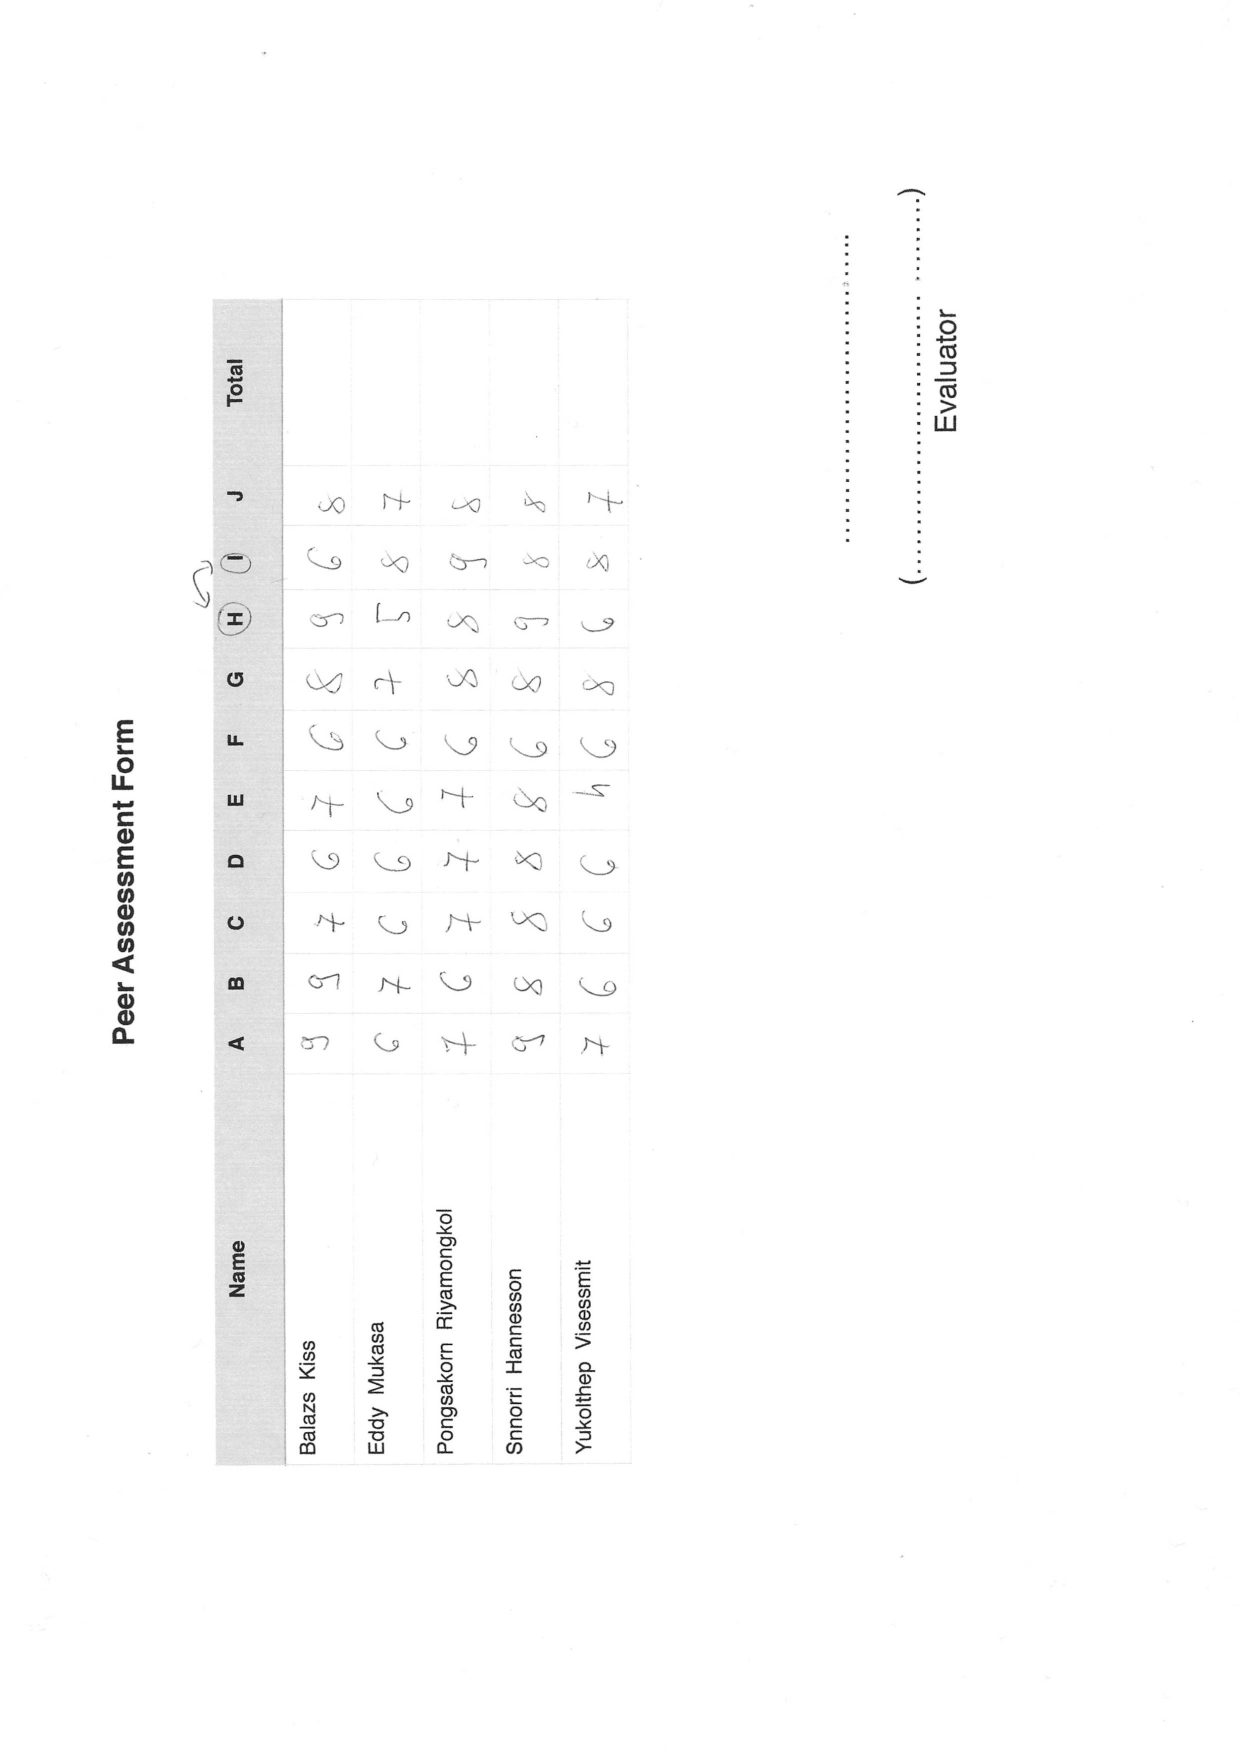
\includepdf[pages=-]{Appendices/peerAssessment/RawAssessment.pdf}
\newpage
% Appendix D: UML

\section{UML design}
\label{AppendixD}

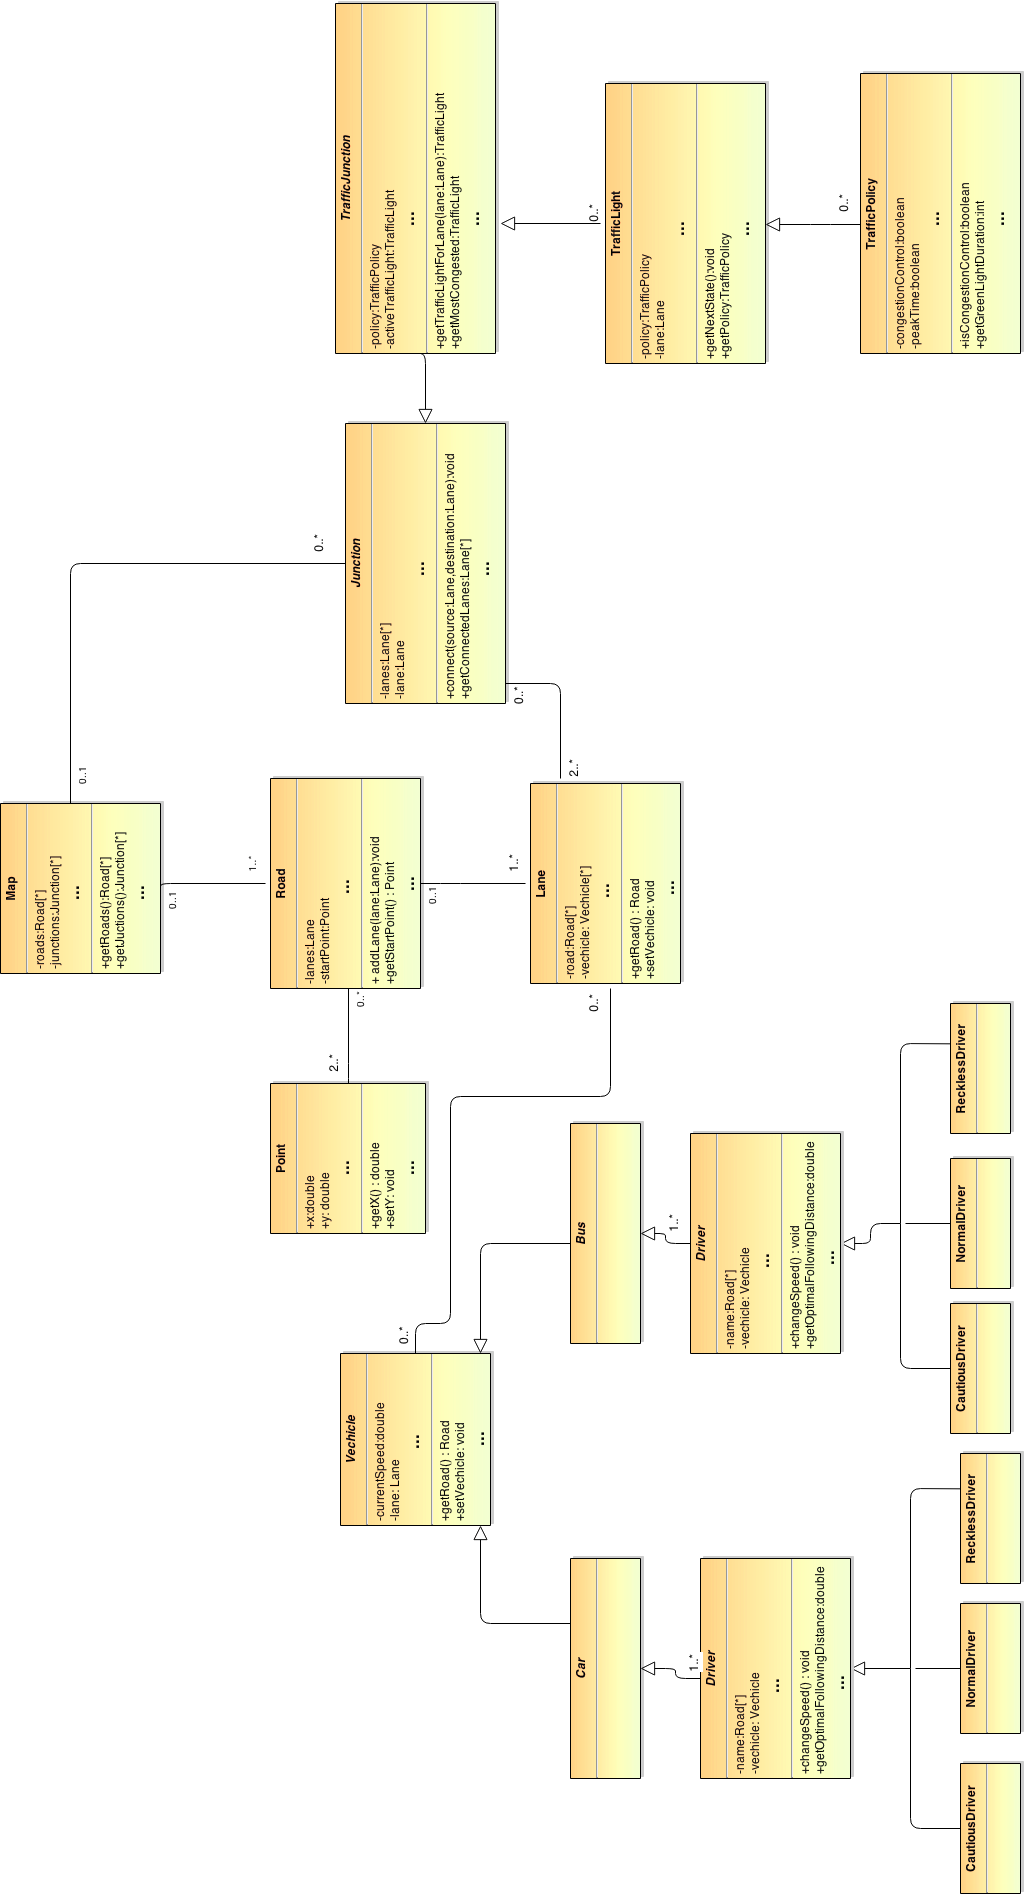
\includegraphics[scale = 0.3]{UML_landscape}






\end{document}
